\section{Results for US influenza hospital admissions}
\label{sec:results}

\subsection{A count-independent floor}
\label{sec:res-floor}

The pooled affine fit of Eq.~\eqref{eq:affine} gave $a=0.0150$ (two-way 95\% CI 0.0109--0.0191; $t_{41}=7.36$, two-sided $p=5.1\times10^{-9}$) and $b=0.560$ (0.430--0.690) (Table~\ref{tab:rev_intercept}). The primary test (E1) rejects $a=0$, and the Holm-adjusted $p$ over the two tests of the plan is $1.0\times10^{-8}$. The secondary calibrations agree. Clustering by state alone or by week alone gave intervals of 0.0125--0.0174 and 0.0112--0.0188. The week-cluster wild bootstrap-$t$ with the null imposed gave $p=0.0001$, the smallest value attainable with 9,999 draws, at every clamp of the bootstrap losses from $10^{-9}$ to $10^{-3}$ and 0.0003 without a clamp (Table~\ref{tab:r2-clamp}). None of the 1,999 calendar-week block-bootstrap draws gave $a\le0$ (block-bootstrap percentile interval 0.0107--0.0192).

The lower limit of $a$ stayed above zero in every sensitivity analysis of the plan, so the claim meets the robustness rule (Fig.~\ref{fig:rev-intercept}). Point estimates ranged from 0.0117 to 0.0202 over 16 independent specifications, and the smallest lower limit, 0.0082, came from leaving out the 2025--26 season. The generation interval moved $a$ most: a mean of 3.2 days gave 0.0117 and a mean of 4.0 days gave 0.0186, because the transform~\eqref{eq:ra} rescales all deviations together. Raising the count floor lowered $a$ slightly, to 0.0130 (0.0088--0.0172) at $C_t\ge50$ on 828 rows. The fixed calendar windows gave the widest interval, 0.0092--0.0311, on 1,263 rows from three seasons. Leaving out one calendar week at a time gave estimates of 0.0136--0.0156 with a smallest lower limit of 0.0100. Count-independent dispersion is therefore present in these data under every specification that the plan fixed, provided the decline with count is inverse; Section~\ref{sec:res-form} examines that proviso.

\begin{table}[!tbp]
\centering
\scriptsize
\setlength{\tabcolsep}{3pt}
\caption{Count-independent intercept $a$: primary test of the analysis plan, secondary calibrations and sensitivity analyses}
\label{tab:rev_intercept}
\begin{tabularx}{\linewidth}{@{}l*{6}{>{\centering\arraybackslash}X}@{}}
\toprule
Analysis (rows) & $a$ & 95\% CI & $t$ & $p$ (two-sided) & $b/a$ & $b/b_P$ \\
\midrule
\multicolumn{7}{l}{\emph{E1, primary: two-way CGM sandwich, $t_{41}$}} \\
All rows (1748) & 0.0150 & 0.0109--0.0191 & 7.36 & $<10^{-4}$ & 37.4 & 1.257 \\
State-cluster sandwich & 0.0150 & 0.0125--0.0174 & 12.23 & $<10^{-4}$ & -- & -- \\
Week-cluster sandwich & 0.0150 & 0.0112--0.0188 & 7.94 & $<10^{-4}$ & -- & -- \\
Week wild bootstrap-$t$, $a=0$ imposed ($B$=9,999) & -- & -- & -- & 0.0001 & -- & -- \\
Calendar-week block bootstrap ($B$=1,999) & -- & 0.0107--0.0192 & -- & -- & 23.4--60.5 & 0.97--1.59 \\
\midrule
\multicolumn{7}{l}{\emph{Sensitivity analyses (two-way sandwich)}} \\
S-a1 GI mean 3.2 (1748) & 0.0117 & 0.0085--0.0149 & 7.44 & $<10^{-4}$ & 37.6 & 1.259 \\
S-a1 GI mean 4.0 (1748) & 0.0186 & 0.0134--0.0237 & 7.27 & $<10^{-4}$ & 37.5 & 1.259 \\
S-a2 GI SD 1.2 (1748) & 0.0154 & 0.0111--0.0197 & 7.27 & $<10^{-4}$ & 37.6 & 1.278 \\
S-a2 GI SD 2.0 (1748) & 0.0144 & 0.0105--0.0183 & 7.46 & $<10^{-4}$ & 37.4 & 1.234 \\
S-a3 count floor 10 (1600) & 0.0140 & 0.0100--0.0180 & 7.07 & $<10^{-4}$ & 46.1 & 1.461 \\
S-a3 count floor 20 (1268) & 0.0136 & 0.0096--0.0176 & 6.82 & $<10^{-4}$ & 48.6 & 1.529 \\
S-a3 count floor 50 (828) & 0.0130 & 0.0088--0.0172 & 6.21 & $<10^{-4}$ & 51.5 & 1.591 \\
S-a4 calendar windows (1263) & 0.0202 & 0.0092--0.0311 & 3.78 & 0.0008 & 25.6 & 1.140 \\
S-a5 threshold 1.02 (1748) & 0.0150 & 0.0109--0.0191 & 7.36 & $<10^{-4}$ & 37.4 & 1.257 \\
S-a5 threshold 1.1 (1564) & 0.0141 & 0.0105--0.0176 & 8.00 & $<10^{-4}$ & 38.6 & 1.255 \\
S-a6 exclude pause (1554) & 0.0139 & 0.0103--0.0176 & 7.76 & $<10^{-4}$ & 41.5 & 1.331 \\
S-a7 drop 2022-23 (1383) & 0.0160 & 0.0105--0.0214 & 5.97 & $<10^{-4}$ & 31.0 & 1.101 \\
S-a7 drop 2023-24 (1249) & 0.0163 & 0.0122--0.0204 & 8.08 & $<10^{-4}$ & 33.3 & 1.240 \\
S-a7 drop 2024-25 (1392) & 0.0152 & 0.0100--0.0204 & 5.89 & $<10^{-4}$ & 36.6 & 1.230 \\
S-a7 drop 2025-26 (1220) & 0.0119 & 0.0082--0.0156 & 6.57 & $<10^{-4}$ & 55.5 & 1.488 \\
S-a8 coverage $\ge$ 90\% (1358) & 0.0159 & 0.0110--0.0207 & 6.59 & $<10^{-4}$ & 31.0 & 1.104 \\
S-a9 leave one week out (42 fits) & 0.0136--0.0156 & min lower 0.0100 & -- & max $<10^{-4}$ & -- & 1.188--1.306 \\
\bottomrule
\end{tabularx}
\par\smallskip\parbox{\linewidth}{\scriptsize\linespread{1.15}\selectfont Robustness rule (locked analysis plan): verdict \emph{robust}; analyses with a lower limit $\le 0$: none. S-a5 with threshold 1.02 reproduces the primary windows. Block-bootstrap columns give percentile intervals.}
\end{table}


\begin{figure}[!tbp]
\centering
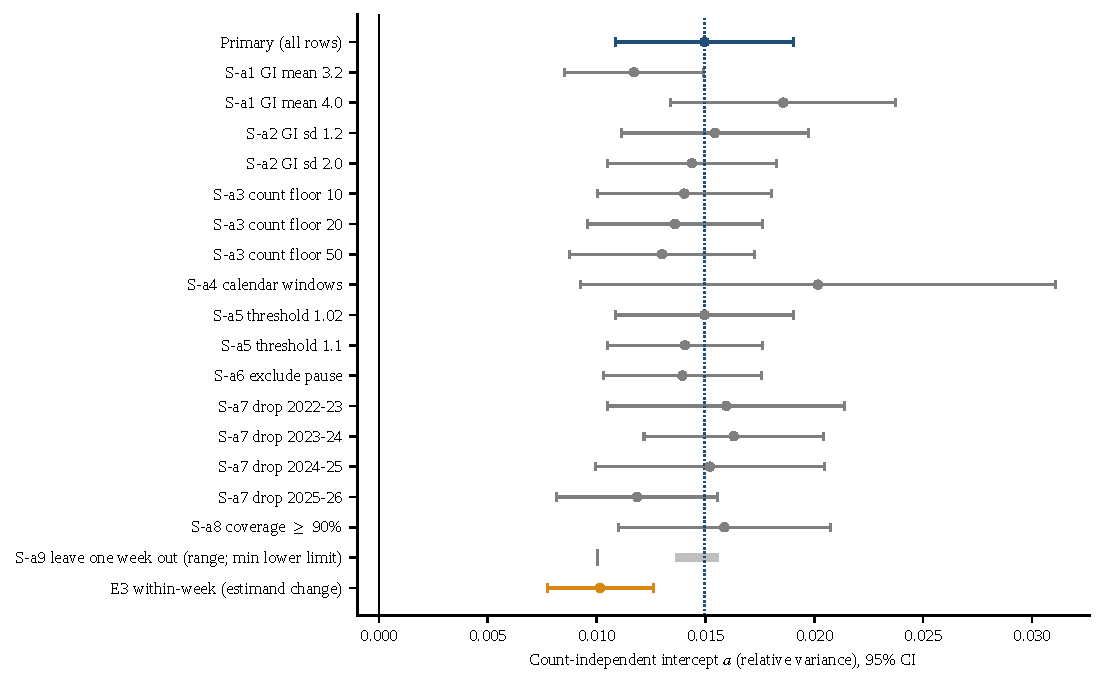
\includegraphics[width=0.92\linewidth]{figures/fig_02_fig_rev_intercept_sens.pdf}
\caption{Count-independent intercept $a$ of the affine dispersion model for $R_A$ under the primary analysis (E1) and sensitivity analyses S-a1 to S-a9, with two-way cluster-robust 95\% confidence intervals. The dotted line marks the primary estimate and the solid line marks zero. For S-a9 the grey bar spans the 42 leave-one-week-out point estimates and the tick marks their smallest lower limit. The within-week intercept (E3, block-bootstrap interval) is a different estimand and is shown for comparison.}
\label{fig:rev-intercept}
\end{figure}

\subsection{How well the affine form fits}
\label{sec:res-form}

The affine form describes the decline of the loss with count only approximately (Table~\ref{tab:r2-deciles}; Fig.~\ref{fig:r2-deciles}). Across deciles of the current-week count the mean loss fell from 0.0684 to 0.0110, and the affine prediction lay outside the block-bootstrap interval of the observed mean in three of ten deciles: above it in the lowest decile (0.0906 against 0.0538--0.0854) and in the highest (0.0158 against 0.0079--0.0137), and below it in the fifth (0.0296 against 0.0310--0.0501). A fit $a+bC^{-\gamma}$ with a free exponent lowered the quasi-deviance by 10.67, and the gain exceeded 2 in 94.6\% of calendar-week block-bootstrap draws (Table~\ref{tab:r2-floor}). Its exponent was $\gamma=0.617$ (week bootstrap 0.355--0.870; state bootstrap 0.438--0.862), so the inverse-count decline $\gamma=1$ lies outside both intervals. Its intercept was 0.0089, and the week-bootstrap interval reached zero ($-0.0014$ to 0.0137; 4.0\% of draws at or below zero), whereas the state-bootstrap interval did not (0.0034--0.0144). Under the reading rule fixed in Amendment~2 the floor therefore does not survive a free exponent. Within the observed counts a slower decline with a smaller constant and an inverse decline with a larger constant describe the data almost equally well, and the intercept of either model is an extrapolation beyond the largest counts.

The rows with the largest counts give the floor without a model for the decline (Table~\ref{tab:r2-floor}; Fig.~\ref{fig:r2-floor}). Among the 175 state-weeks at or above the 90th percentile of the count ($C_t\ge389$, mean 882) the mean loss was 0.0110 (week bootstrap 0.0078--0.0139), a relative root mean squared deviation of 10.5\% (8.8--11.8\%). Subtracting the counting term with the fitted slope left 0.0102 (0.0069--0.0132), a relative standard deviation of 10.1\% (8.3--11.5\%), and subtracting it with the Poisson reference left 0.0104 (0.0071--0.0132). At the 75th and 95th percentiles the net relative standard deviation was 11.8\% (9.8--13.2\%) and 9.8\% (8.0--11.1\%). At the largest observed counts, therefore, a count-independent relative error of about 10\% remains, and all of these intervals exclude zero. The model-free value at the 90th percentile lies between the three-parameter intercept and the affine one.

\begin{figure}[!tbp]
\centering
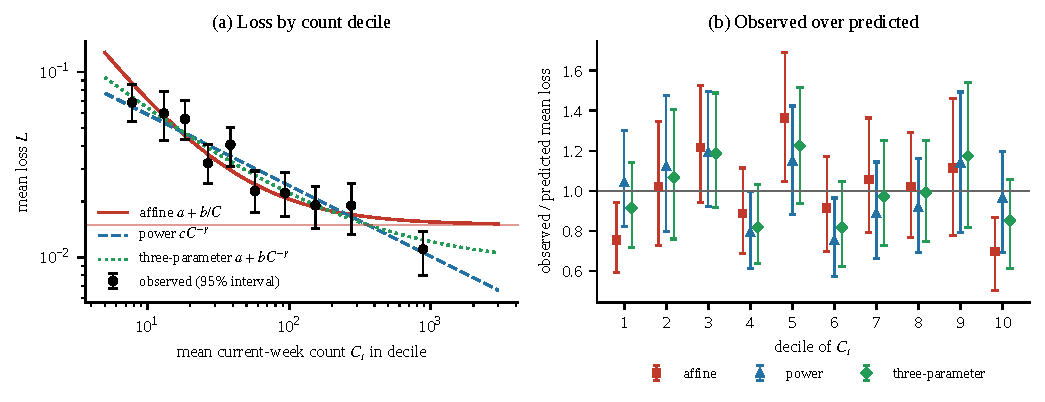
\includegraphics[width=0.98\linewidth]{figures/fig_03_deciles.pdf}
\caption{Loss by decile of the current-week count. (A) Mean relative squared deviation $L$ against mean count $C_t$ on log scales, with calendar-week block-bootstrap 95\% intervals (1,999 draws). Lines show the fitted affine ($a+b/C$), power ($cC^{-\gamma}$) and three-parameter ($a+bC^{-\gamma}$) curves. (B) Ratio of the observed mean loss to the prediction of each model by decile; the dotted line marks 1.}
\label{fig:r2-deciles}
\end{figure}

\begin{table}[!tbp]
\centering
\scriptsize\renewcommand{\arraystretch}{1.15}
\setlength{\tabcolsep}{3pt}
\caption{The floor under a free exponent and without a model}
\label{tab:r2-floor}
\begin{tabularx}{\linewidth}{@{}Xrll@{}}
\toprule
Quantity & Estimate & Week bootstrap & State bootstrap \\
\midrule
\multicolumn{4}{@{}l}{\textit{Affine fit $a+b/C$ (primary, for reference)}} \\
$a$ (two-way interval) & 0.0150 & 0.0109--0.0191 & -- \\
\midrule
\multicolumn{4}{@{}l}{\textit{Three-parameter fit $a+bC^{-\gamma}$}} \\
$a$ & 0.0089 & $-$0.0014 to 0.0137 & 0.0034--0.0144 \\
$b$ & 0.228 & 0.130--0.436 & -- \\
$\gamma$ & 0.617 & 0.355--0.870 & 0.438--0.862 \\
Share of draws with $a\le 0$ & -- & 0.040 & 0.006 \\
Quasi-deviance gain over affine & 10.67 & share $>2$: 0.946 & -- \\
\midrule
\multicolumn{4}{@{}l}{\textit{Model-free floor among rows with $C_t$ at or above a quantile}} \\
P75 ($C_t\ge 152$, $n=438$, mean $C_t$ 497): mean $L$ & 0.0157 & 0.0117--0.0191 & -- \\
\quad mean $L-\hat b/C_t$ & 0.0139 & 0.0096--0.0176 & -- \\
\quad mean $L-b_P/C_t$ & 0.0142 & 0.0102--0.0177 & -- \\
\quad relative SD $(L-\hat b/C_t)^{1/2}$ (\%) & 11.8 & 9.8--13.2 & -- \\
P90 ($C_t\ge 389$, $n=175$, mean $C_t$ 882): mean $L$ & 0.0110 & 0.0078--0.0139 & -- \\
\quad mean $L-\hat b/C_t$ & 0.0102 & 0.0069--0.0132 & -- \\
\quad mean $L-b_P/C_t$ & 0.0104 & 0.0071--0.0132 & -- \\
\quad relative SD $(L-\hat b/C_t)^{1/2}$ (\%) & 10.1 & 8.3--11.5 & -- \\
P95 ($C_t\ge 699$, $n=90$, mean $C_t$ 1238): mean $L$ & 0.0101 & 0.0071--0.0128 & -- \\
\quad mean $L-\hat b/C_t$ & 0.0096 & 0.0064--0.0123 & -- \\
\quad mean $L-b_P/C_t$ & 0.0097 & 0.0066--0.0124 & -- \\
\quad relative SD $(L-\hat b/C_t)^{1/2}$ (\%) & 9.8 & 8.0--11.1 & -- \\
\bottomrule
\end{tabularx}
\par\smallskip\parbox{\linewidth}{\scriptsize\linespread{1.15}\selectfont Week bootstrap: calendar-week blocks (1,999 draws); state bootstrap: states resampled (999 draws). Model-free floor: mean loss of the rows above the threshold minus the mean counting term, with $\hat b$ the fitted slope or $b_P$ the Poisson reference; intervals from the calendar-week block bootstrap with $\hat b$ refitted in each draw. Reading rule of Amendment 2: the floor survives a free exponent if the week-bootstrap interval of $a$ excludes 0 (here: no).}
\end{table}


\begin{figure}[!tbp]
\centering
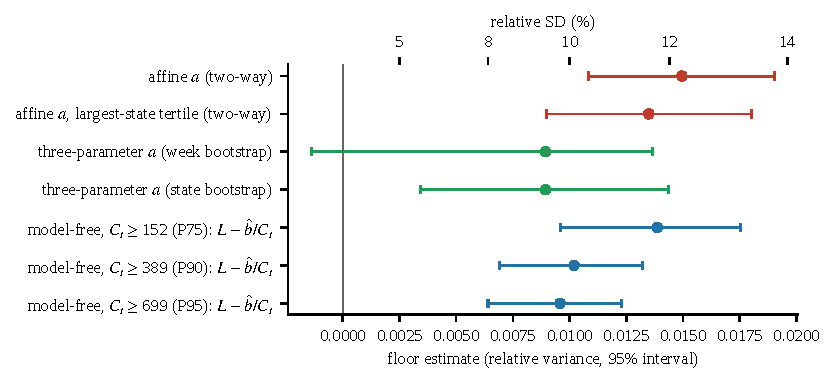
\includegraphics[width=0.92\linewidth]{figures/fig_04_floor.pdf}
\caption{Estimates of the count-independent component on the relative-variance scale, with the corresponding relative standard deviation on the upper axis. Rows show the affine intercept (two-way cluster-robust 95\% interval), the same intercept in the largest-population tertile (two-way interval) and the three-parameter intercept with calendar-week and state bootstrap 95\% intervals. The remaining rows show the model-free floor (mean loss minus the fitted counting term) among rows at or above the 75th, 90th and 95th percentiles of the count, with calendar-week block-bootstrap 95\% intervals. The solid line marks zero.}
\label{fig:r2-floor}
\end{figure}

\subsection{What more cases buy}
\label{sec:res-buy}

The observed relative error fell with count but levelled off at large counts (Table~\ref{tab:r2-deciles}). The relative root mean squared deviation of $R_A$ was 26.2\% in the lowest count decile (mean 7.8 admissions a week), 20.1\% in the fifth (mean 38.5), 14.9\% in the seventh (mean 93.5) and 10.5\% in the highest (mean 882). A ninefold increase in the mean count from the seventh to the tenth decile thus lowered the relative error by about four percentage points. The affine model gives smooth values over the same range, 26.6\% at 10 admissions, 17.3\% at 37 and 14.3\% at 100 (Table~\ref{tab:rev_error_components}). Its extrapolation to 1,000 admissions, 12.5\%, exceeds the observed relative error of the highest decile, so statements about large counts here rest on the model-free floor of Section~\ref{sec:res-form}. The crossover count, at which the two affine terms are equal, was $b/a=37.4$ admissions a week (two-way 24.1--58.3; block bootstrap 23.4--60.5). It rose to 46.1, 48.6 and 51.5 at count floors of 10, 20 and 50 and lay between 25.6 and 55.5 across the other sensitivity analyses, so its order of magnitude, a few tens of weekly admissions, is stable while its value is not. It is an in-sample balance point for this panel, not a sample-size rule for surveillance.

These values pool jurisdictions whose count-independent component differs (Section~\ref{sec:res-pop}). Separate affine fits by population tertile gave predicted relative errors at 37, 100 and 390 admissions of 18.3, 15.6 and 14.2\% in the smallest-population tertile, 17.9, 15.5 and 14.4\% in the middle tertile and 16.2, 13.5 and 12.1\% in the largest. What additional cases buy should be judged against the component of the jurisdiction concerned.

\begin{table}[!tbp]
\centering
\scriptsize
\setlength{\tabcolsep}{3pt}
\caption{What more cases buy: predicted relative squared error $a+b/C$ by count, crossover, and the within-week intercept}
\label{tab:rev_error_components}
\begin{tabularx}{\linewidth}{@{}r*{7}{>{\centering\arraybackslash}X}@{}}
\toprule
$C$ & $a$ & $b/C$ & $a+b/C$ & 95\% CI (sandwich) & 95\% CI (block bootstrap) & Share from $a$ (\%) & Relative RMSE (\%) \\
\midrule
10 & 0.0150 & 0.0560 & 0.0710 & 0.0595--0.0824 & 0.0604--0.0829 & 21.1 & 26.6 \\
37 & 0.0150 & 0.0151 & 0.0301 & 0.0263--0.0339 & 0.0264--0.0333 & 49.7 & 17.3 \\
100 & 0.0150 & 0.0056 & 0.0206 & 0.0170--0.0242 & 0.0168--0.0239 & 72.8 & 14.3 \\
1,000 & 0.0150 & 0.0006 & 0.0155 & 0.0115--0.0196 & 0.0113--0.0196 & 96.4 & 12.5 \\
\midrule
\multicolumn{8}{l}{Crossover $C^\times=b/a$ = 37.4; sandwich (log-delta) 24.1--58.3; block bootstrap 23.4--60.5} \\
\midrule
\multicolumn{8}{l}{\emph{Within-week intercept (E3, estimand change; block bootstrap 95\% CI)}} \\
\multicolumn{3}{l}{Leave-state-out week centre (primary)} & 0.0102 & 0.0078--0.0126 & \multicolumn{3}{c}{share of $a$ removed 32.0\% (10.2--47.8)} \\
\multicolumn{3}{l}{Week centre incl. own row} & 0.0098 & 0.0075--0.0121 & \multicolumn{3}{c}{share of $a$ removed 34.7\% (13.8--49.8)} \\
\multicolumn{3}{l}{Week centre and scale} & 0.0086 & 0.0066--0.0107 & \multicolumn{3}{c}{share of $a$ removed 42.6\% (22.0--57.0)} \\
\multicolumn{3}{l}{Season centre} & 0.0147 & 0.0101--0.0184 & \multicolumn{3}{c}{share of $a$ removed 1.6\% ($-$6.8 to 19.1)} \\
\multicolumn{3}{l}{Pooled centre (E1 loss)} & 0.0150 & 0.0107--0.0191 & \multicolumn{3}{c}{share of $a$ removed 0.0\% (0.0--0.0)} \\
\bottomrule
\end{tabularx}
\end{table}


\subsection{Jurisdiction size}
\label{sec:res-pop}

The intercept fell with state population (Table~\ref{tab:r2-population}; Fig.~\ref{fig:r2-population}). In the Amendment~2 model with an intercept linear in standardised log population and a common slope, the population coefficient was $a_1=-0.0054$ per standard deviation (two-way $-0.0085$ to $-0.0023$; $t_{41}=-3.51$, $p=0.0011$), and its state-bootstrap and week-bootstrap intervals also excluded zero. The fitted intercept was 0.0273 at the 10th percentile of population (0.92 million) and 0.0137 at the 90th (12.7 million), a ratio of 0.50 (state bootstrap 0.41--0.61); a log-link intercept gave a ratio of 0.44 (state bootstrap 0.32--0.60). The counting slope did not change detectably with population (coefficient $-0.015$; two-way $-0.124$ to 0.095). Separate fits by tertile gave intercepts of 0.0189 (two-way 0.0145--0.0233), 0.0195 (0.0125--0.0264) and 0.0135 (0.0090--0.0180), and with a common slope the ratio of the largest-population to the smallest-population tertile was 0.60 (state bootstrap 0.42--0.82).

Whether that gradient survives a freer count law was tested in Amendment~3. Refitting both the linear-population model and a free-exponent model that replaces $b/C_t$ by $bC_t^{-\gamma}$ gave $a_1=-0.0048$ per standard deviation in the free-exponent model (two-way $-0.0080$ to $-0.0017$; $t_{41}=-3.08$, $p=0.0037$), and the state bootstrap for $a_1$ gave $-0.0074$ to $-0.0027$. The implied intercept ratio between the 10th and 90th population percentiles was 0.50 in the affine model and 0.49 in the free-exponent model (state bootstrap 0.40--0.61), with $\gamma=0.79$ (state bootstrap 0.57--1.09). The gradient is therefore not an artefact of forcing an inverse count law.

Population and count go together in this panel: the median count was 20, 37 and 106 admissions in the three tertiles. Because the affine form overpredicts the loss at the largest counts (Section~\ref{sec:res-form}), part of the population gradient may reflect that misfit rather than a property of the jurisdictions. Either way the pooled intercept of 0.0150 is an average over jurisdictions whose count-independent component differs about twofold, and the count beyond which more cases help little is specific to the jurisdiction.

\begin{table}[!tbp]
\centering
\scriptsize\renewcommand{\arraystretch}{1.15}
\setlength{\tabcolsep}{3pt}
\caption{Dependence of the count-independent intercept on state population}
\label{tab:r2-population}
\begin{tabularx}{\linewidth}{@{}Xrlll@{}}
\toprule
Quantity & Estimate & Two-way & State bootstrap & Week bootstrap \\
\midrule
\multicolumn{5}{@{}l}{\textit{Linear intercept $a_0+a_1z$, common slope $b$ (primary)}} \\
$a_0$ & 0.0197 & 0.0136--0.0258 & -- & -- \\
$a_1$ (per SD of log population) & $-$0.0054 & $-$0.0085 to $-$0.0023 & $-$0.0078 to $-$0.0034 & $-$0.0085 to $-$0.0023 \\
$a$ at population P10 / P90 & 0.0273 / 0.0137 & -- & -- & -- \\
Ratio $a$(P90) / $a$(P10) & 0.501 & -- & 0.408--0.609 & -- \\
$b$ & 0.451 & -- & -- & -- \\
\midrule
\multicolumn{5}{@{}l}{\textit{Log-link intercept $\exp(\alpha_0+\theta z)$ (secondary)}} \\
$\theta$ & $-$0.327 & -- & $-$0.445 to $-$0.205 & $-$0.438 to $-$0.183 \\
Ratio $a$(P90) / $a$(P10) & 0.436 & -- & 0.324--0.595 & -- \\
\midrule
\multicolumn{5}{@{}l}{\textit{Intercept and slope both linear in $z$ (secondary)}} \\
$a_1$ & $-$0.0052 & $-$0.0083 to $-$0.0022 & -- & -- \\
$b_1$ & $-$0.015 & $-$0.124 to 0.095 & -- & -- \\
\midrule
\multicolumn{5}{@{}l}{\textit{Population tertiles, separate affine fits (two-way interval, $t$ with $G-1$ df)}} \\
Tertile 1 (17 states, 0.59--2.9 M, 399 rows): $a$ & 0.0189 & 0.0145--0.0233 & -- & -- \\
\quad $b$ (median $C_t$ = 20) & 0.534 & 0.350--0.719 & -- & -- \\
Tertile 2 (17 states, 2.96--6.2 M, 638 rows): $a$ & 0.0195 & 0.0125--0.0264 & -- & -- \\
\quad $b$ (median $C_t$ = 37) & 0.462 & 0.299--0.624 & -- & -- \\
Tertile 3 (17 states, 6.91--39.3 M, 711 rows): $a$ & 0.0135 & 0.0090--0.0180 & -- & -- \\
\quad $b$ (median $C_t$ = 106) & 0.475 & 0.218--0.732 & -- & -- \\
\midrule
\multicolumn{5}{@{}l}{\textit{Population tertiles, common slope}} \\
Tertile 1 intercept & 0.0213 & -- & 0.0160--0.0303 & -- \\
Tertile 2 intercept & 0.0191 & -- & 0.0149--0.0240 & -- \\
Tertile 3 intercept & 0.0128 & -- & 0.0105--0.0158 & -- \\
Ratio tertile 3 / tertile 1 & 0.601 & -- & 0.421--0.818 & -- \\
\bottomrule
\end{tabularx}
\par\smallskip\parbox{\linewidth}{\scriptsize\linespread{1.15}\selectfont $z$: log of the mean 2022--2025 resident population (Census Vintage 2025), standardised over the 51 jurisdictions (P10 = 0.92 M, P90 = 12.7 M). Primary test of $a_1=0$: two-way sandwich, $t$ with 41 df, $t=-3.51$, $p=0.0011$. State bootstrap: states resampled (1,999 draws; 999 for the tertile fits); week bootstrap: calendar-week blocks (1,999 draws). All intervals 95\%.}
\end{table}


\begin{figure}[!tbp]
\centering
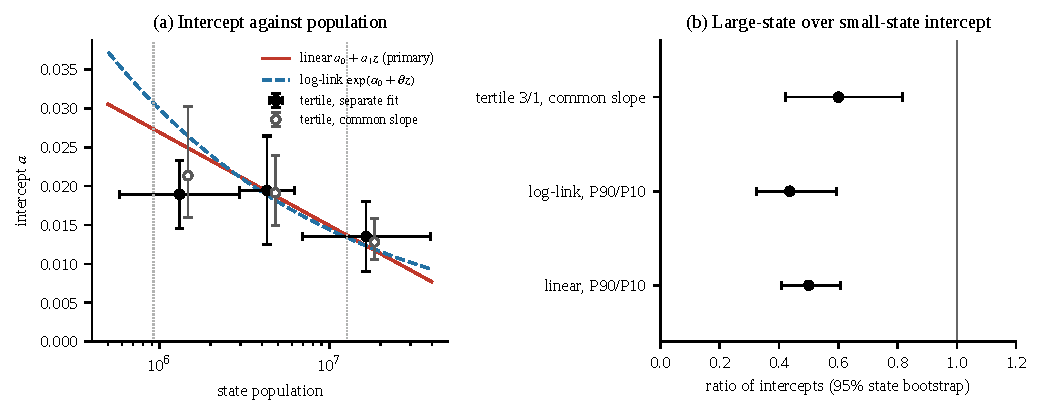
\includegraphics[width=0.98\linewidth]{figures/fig_05_population.pdf}
\caption{Count-independent intercept and state population. (A) Fitted intercept against mean resident population for the linear and log-link population models, with separate affine fits by population tertile (filled points, two-way cluster-robust 95\% intervals) and tertile intercepts under a common slope (open points). Dotted lines mark the 10th and 90th percentiles of population. (B) Ratios of intercepts with state-bootstrap 95\% intervals: 90th to 10th percentile of population under the linear and log-link models, and largest to smallest tertile under a common slope.}
\label{fig:r2-population}
\end{figure}

\subsection{What the floor contains}
\label{sec:res-content}

Removing common national variation by calendar week lowered the intercept to 0.0102 (block bootstrap 0.0078--0.0126) with the leave-state-out week centre, a reduction of 32.0\% (10.2--47.8) (Table~\ref{tab:rev_error_components}). With the week centre including the own row the reduction was 34.7\% (13.8--49.8), and with week-specific centre and scale it was 42.6\% (22.0--57.0). Centring by season removed 1.6\% ($-6.8$ to 19.1). About a third of the floor is thus shared by states in the same week, and about two thirds varies between states within a week. The within-week intercept stays above zero under every centring.

The floor reflects transmission and reporting variation, and its transmission share is not identified. The square root of $a$, 12.2\%, is the relative standard deviation of the non-counting variation that the intercept captures around the pooled mean, which can fall short of the sum of the two sources (Section~\ref{sec:res-bias}). Converting $a$ into a transmission standard deviation requires a mechanism, and across 71 simulated mechanisms the implied relative standard deviation of the reproduction number ranged from 8.6\% to 18.6\%, with propagated intervals from 6.9\% to 22.7\% (Table~\ref{tab:rev_implied_sd}; Fig.~\ref{fig:rev-implied-sd}). Restricted to the 13 mechanisms that reproduce the observed counting slope, the range was 8.6--13.9\%. Reporting shocks make the intercept overstate transmission variance, and heterogeneity that shrinks with count makes it understate it, which is why the range is wide in both directions.

The mapping itself depends on the time scale of transmission (SC1). Under a daily renewal process with the primary generation interval, about two generations fall within a week, and the intercept recovered 75--78\% of the variance of the weekly reproduction number, outside the range of 0.8--1.25 fixed in the plan. Against the mean of two consecutive weekly values it recovered 150--156\%. The one-generation map of Section~\ref{sec:model} therefore does not carry over unchanged to weekly hospital counts, and the implied standard deviations above inherit this dependence.

\begin{table}[!tbp]
\centering
\scriptsize
\setlength{\tabcolsep}{3pt}
\caption{Implied relative SD of the reproduction number across simulated mechanisms (a grid, not an estimate)}
\label{tab:rev_implied_sd}
\begin{tabularx}{\linewidth}{@{}X c c c c c@{}}
\toprule
Mechanism family & Rows & Point range (\%) & Interval envelope (\%) & Reproduce $b/b_P$ & Post hoc laws \\
\midrule
original generators (fixed field) & 9 & 8.6--18.6 & 6.9--22.7 & 4 & 1 \\
fresh-draw generator & 5 & 9.2--12.1 & 7.1--14.7 & 4 & 3 \\
$\rho\times k$ grid (S1 field) & 40 & 10.0--12.3 & 7.5--14.5 & 3 & 0 \\
daily renewal (two generations per week) & 12 & 9.8--14.1 & 7.8--17.2 & 2 & 0 \\
generation-interval variant ($r=1$) & 4 & 10.8--13.6 & 9.2--15.4 & -- & 0 \\
within-week estimand (E3, $r=1$) & 1 & 10.1--10.1 & 8.8--11.2 & -- & 0 \\
\midrule
\emph{All rows} & 71 & 8.6--18.6 & 6.9--22.7 & -- & -- \\
\emph{Pre-specified laws} & 67 & 8.6--18.6 & 6.9--22.7 & -- & -- \\
\emph{Rows reproducing $b/b_P$} & 13 & 8.6--13.9 & 6.9--17.1 & -- & -- \\
\bottomrule
\end{tabularx}
\par\smallskip\parbox{\linewidth}{\scriptsize\linespread{1.15}\selectfont Implied SD $=\sqrt{a_{\mathrm{obs}}/r}$, $r=E(\hat a)/v_R$ of each mechanism; intervals combine the two-way CI of $a$ with the MC 2.5--97.5\% range of $r$. The transmission share of $a$ is not identified. Renewal rows appear twice (following-week $R$ and two-week mean $R$).}
\end{table}


\begin{figure}[!tbp]
\centering
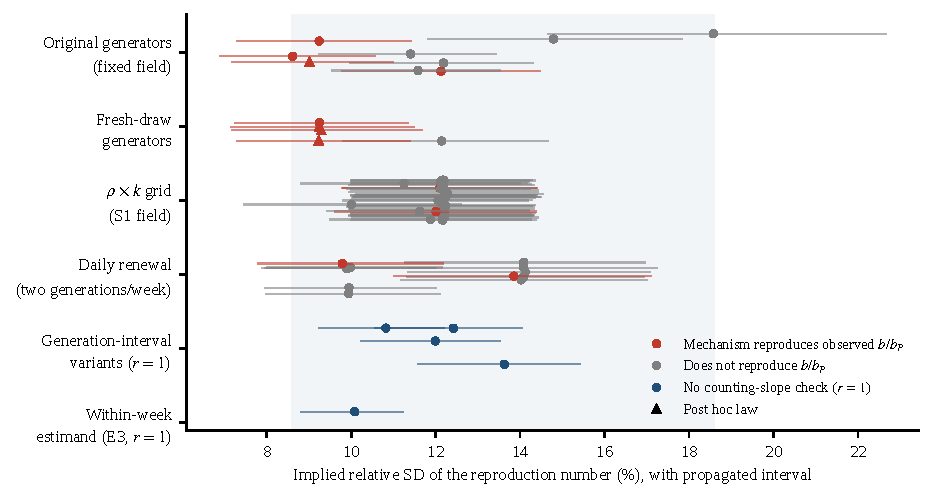
\includegraphics[width=0.95\linewidth]{figures/fig_06_implied_sd.pdf}
\caption{Relative standard deviation of the reproduction number implied by the observed intercept, $(a/r)^{1/2}$, for each simulated mechanism with recovery ratio $r=\E(\hat a)/v_R$, grouped by mechanism family. Bars combine the two-way 95\% interval of $a$ with the Monte Carlo 2.5--97.5\% range of $r$. Red points mark mechanisms whose Monte Carlo range of $b/\bP$ contains the observed value, grey points those that do not, and blue points rows with $r=1$ for which no slope check applies; triangles mark laws defined after the data had been seen. The shaded band spans the point values of all rows. Daily-renewal rows appear twice, against the following-week and the two-week mean reproduction number.}
\label{fig:rev-implied-sd}
\end{figure}

\subsection{How the intercept relates to its sources}
\label{sec:res-bias}

Under fresh-draw generators the intercept tracked transmission variance when there was no reporting shock and fell short of the total when there was (Table~\ref{tab:r2-bias}). With independent heterogeneity (FD-S1) its relative bias against $v_R+v_H$ was $+1.4\%$ (panel bootstrap 0.5--2.3\%). Under FD-S8, in which about half of the calibrated variance is a reporting shock, it was $-14.2\%$ ($-15.1$ to $-13.3\%$), and under the three post hoc variants FD-S9 it was $-13.8$ to $-14.9\%$. Varying the transmission share of the FD-S8 variance moved the shortfall from 22.1\% at a share of 0.75 to 6.3\% at a share of 0.25, and with no reporting shock in that family the intercept recovered 0.707 of the transmission variance. The weight of the reporting variance in $\E(\hat a)=v_R+w_Hv_H$ ranged from 0.10 to 0.91 across these laws. The direction of the bias is downward under every law with reporting shocks, and its size depends on the share and mechanism, neither of which the data identify. The intercept is therefore not rescaled, which would give 0.0160--0.0192 depending on the law, and it is read as reflecting transmission and reporting variation rather than as an estimate of their sum.

\begin{table}[!tbp]
\centering
\scriptsize\renewcommand{\arraystretch}{1.15}
\setlength{\tabcolsep}{3pt}
\caption{Bias of the intercept relative to the total non-counting variance}
\label{tab:r2-bias}
\begin{tabularx}{\linewidth}{@{}Xrrrrlrl@{}}
\toprule
Generator & $v_H$ share (\%) & $E(\hat a)$ & $v_R$ & $v_H$ & Rel. bias (\%) & $E(\hat a)/v_R$ & $w_H$ \\
\midrule
FD-S1 & 0.0 & 0.0149 & 0.0146 & 0.0000 & 1.4 (0.5--2.3) & 1.014 & -- \\
FD-S8 & 50.9 & 0.0150 & 0.0086 & 0.0089 & $-$14.2 ($-$15.1 to $-$13.3) & 1.749 & 0.708 (0.687--0.729) \\
FD-S9, 25$^\dagger$ & 50.9 & 0.0151 & 0.0086 & 0.0089 & $-$13.8 ($-$14.8 to $-$12.8) & 1.754 & 0.715 (0.693--0.736) \\
FD-S9, 50$^\dagger$ & 50.9 & 0.0150 & 0.0086 & 0.0089 & $-$14.0 ($-$15.1 to $-$12.9) & 1.753 & 0.711 (0.689--0.734) \\
FD-S9, 75$^\dagger$ & 50.8 & 0.0148 & 0.0086 & 0.0089 & $-$14.9 ($-$16.1 to $-$13.7) & 1.731 & 0.693 (0.669--0.718) \\
FD-S8, share 100 & 0.0 & 0.0154 & 0.0217 & 0.0000 & $-$29.3 ($-$30.1 to $-$28.4) & 0.707 & -- \\
FD-S8, share 75 & 25.7 & 0.0152 & 0.0144 & 0.0050 & $-$22.1 ($-$23.1 to $-$21.2) & 1.049 & 0.100 (0.056--0.147) \\
FD-S8, share 25 & 75.6 & 0.0148 & 0.0039 & 0.0120 & $-$6.3 ($-$7.2 to $-$5.4) & 3.840 & 0.912 (0.900--0.924) \\
\bottomrule
\end{tabularx}
\par\smallskip\parbox{\linewidth}{\scriptsize\linespread{1.15}\selectfont Fresh-draw generators of the first revision (200 panels each) and an FD-S8 sweep over the transmission share of the calibrated variance (shares 1.0, 0.75, 0.25; 0.5 is FD-S8 itself). $v_R$, $v_H$: true relative variance of transmission and of the reporting shock on the kept rows; relative bias $=E(\hat a)/(v_R+v_H)-1$; $w_H$: weight on $v_H$ solving $E(\hat a)=v_R+w_Hv_H$. Intervals: panel bootstrap (2,000 draws). $^\dagger$ post hoc law. Wording rule of Amendment 2: if every interval excludes 0, the manuscript says $\hat a$ reflects, not estimates, the total (outcome: reflects (not an estimate of the total)). Mechanism-conditional rescaling $a_{\mathrm{obs}}/t_g$ would range 0.0160--0.0192; not used.}
\end{table}


\subsection{External reporting data}
\label{sec:res-reporting}

Two external sources bound parts of the reporting component (Table~\ref{tab:r2-reporting}). Hospital participation averaged 92.9\% of hospitals per jurisdiction-week (minimum 67.7\%) and changed by 0.78 percentage points between consecutive weeks on average. Scaling both counts by participation lowered $a$ by 0.00029, or 2.0\% (week bootstrap $-0.00086$ to 0.00027), so changing participation explains little of the intercept. Revisions explain more. In the Delphi Epidata archive of issues \citep{reinhart2021open}, which starts with week 47 of 2024, 661 rows had a provisional first issue in both weeks. The first issue equalled the latest in 29.2\% of them, was revised upward in 65.8\% and downward in 5.0\%, and the mean relative revision was 11.0\%. On the 654 rows with both counts at least 5, $a$ was 0.0227 (block bootstrap 0.0133--0.0298) with first-issue counts and 0.0143 (0.0096--0.0183) with latest-issue counts, a difference of 0.0084 (0.0016--0.0146). Counts available in real time thus carry a count-independent component about 1.6 times that of settled counts. Neither source measures the reporting error that remains in settled counts, so the transmission share of $a$ stays unidentified.

\begin{table}[!tbp]
\centering
\scriptsize\renewcommand{\arraystretch}{1.15}
\setlength{\tabcolsep}{3pt}
\caption{External reporting data: participation and backfill}
\label{tab:r2-reporting}
\begin{tabularx}{\linewidth}{@{}Xll@{}}
\toprule
Quantity & Value & 95\% interval \\
\midrule
\multicolumn{3}{@{}l}{\textit{Hospital participation (NHSN, \% of hospitals reporting)}} \\
Mean (min; P10) participation & 92.9\% (67.7; 86.9) & -- \\
Rows with full participation in both weeks & 4.1\% & -- \\
Mean week-to-week change & 0.78 pp & -- \\
$a$, observed counts & 0.0150 & -- \\
$a$, participation-adjusted counts & 0.0147 & two-way SE 0.0020 \\
Difference (relative) & $-$0.00029 ($-$2.0\%) & $-$0.00086 to 0.00027 \\
\midrule
\multicolumn{3}{@{}l}{\textit{Backfill (Delphi Epidata issue history, archive from issue 2024w47)}} \\
Rows of $R_A$ in the archive; latest issue equals the vintage & 1,748; 99.1\% & -- \\
Rows with a provisional first issue (lag $\le$ 2 weeks) & 661 (15 weeks, 2024-11-09 to 2025-12-27) & -- \\
First issue equals latest (current week) & 29.2\% & -- \\
Revised up / down & 65.8\% / 5.0\% & -- \\
Mean relative revision (latest $-$ first) / first & 11.0\% & -- \\
$a$, latest issue (654 rows) & 0.0143 & 0.0096--0.0183 \\
$a$, first issue & 0.0227 & 0.0133--0.0298 \\
Difference first $-$ latest & 0.0084 & 0.0016--0.0146 \\
$v_{\mathrm{rev}}$ (revision variance of $x$) & 0.0107 & -- \\
\bottomrule
\end{tabularx}
\par\smallskip\parbox{\linewidth}{\scriptsize\linespread{1.15}\selectfont Participation adjustment: both counts scaled by 100/participation, $x$ recomputed, the affine fit repeated with the observed $C_t$ as the count; assumes unreported hospitals admit as many patients per hospital as reporting ones. Backfill: rows whose two weeks both have a provisional first issue; fits restricted to rows with first and latest counts $\ge 5$. Intervals: calendar-week block bootstrap, 1,999 draws. The backfill comparison bounds the provisional-versus-settled component only; the residual reporting error of the settled vintage is not identified from public data.}
\end{table}


\subsection{Counting slope, reporting and offspring dispersion}
\label{sec:res-slope}

The counting slope was 1.257 times the plug-in independent-Poisson reference $\bP$. That reference normalises every row by the squared pooled mean; normalising each row by its own ratio to the pooled mean lowers $\bP$ from 0.4455 to 0.4199 and raises the ratio by 6.1\% to 1.334. An exact reference simulated from Poisson counts on the same design gives 0.3977 and a ratio of 1.408 (Table~
ef{tab:r2-poisson}). All three intervals below resample calendar weeks and recompute the reference in every draw (B~=~1,999): 0.96--1.61 under the plug-in reference, 1.04--1.67 under the row-normalised one and 1.08--1.81 under the simulated exact one, with 4.3\%, 1.5\% and 0.7\% of draws at or below 1 (Table~
ef{tab:r2-poisson}). Whether counting variation exceeds independent Poisson noise therefore depends on the reference: the interval excludes 1 under the two closer approximations but not under the plug-in reference used in the plan. The three references are not nested, so no single one settles the question. The comparisons with simulated slopes below use the plug-in reference throughout, so they are not affected. Against the branching-Poisson reference of Eq.~\eqref{eq:branching-reference} the point ratio would be 1.46 at $\rho=0.25$ and 2.84 at $\rho=1$ (Table~\ref{tab:ma_baselines}), but the slope does not identify $\rho$. Within-state fits were less precise: a state fixed-effects fit gave 0.85 (0.24--1.47) times $\bP$ and a week fixed-effects fit 1.42 (0.96--1.89) (Table~\ref{tab:ma_within}).

The reporting-by-offspring grid shows what the slope can and cannot reveal (Table~\ref{tab:rev_rho_grid}; Fig.~\ref{fig:rev-rho-grid}). Intercept recovery stayed within 0.9--1.1 at $\rho\le0.25$ for every offspring law and at all $\rho$ for $k\ge1$, but rose to 1.18 at $\rho=0.5$ and 1.49 at $\rho=1$ with $k=0.1$, and to 1.11 at $\rho=1$ with $k=0.3$; SC2 therefore fails, in cells outside the assumed range of $\rho$. In the assumed range, $\rho\le0.01$, the expected slope ratio was 0.85--0.91 whatever the offspring law, below 1 rather than within 0.9--1.1 as SC3 required. Offspring dispersion cannot be read from the counting slope at realistic reporting probabilities, and no cell in that range reproduces the observed 1.257. Only three of 40 cells did, all with $\rho\ge0.1$ and $k\le0.3$. The observed slope is thus compatible with strong overdispersion only at reporting probabilities far above those of hospital surveillance, or with counting variation that the simulated mechanisms do not contain.

\begin{table}[!tbp]
\centering
\scriptsize\renewcommand{\arraystretch}{1.15}
\setlength{\tabcolsep}{3pt}
\caption{Counting slope against three Poisson references}
\label{tab:r2-poisson}
\begin{tabularx}{\linewidth}{@{}Xrrlr@{}}
\toprule
Reference & $b_P$ & $b/b_P$ & 95\% interval & Change vs.\ shipped (\%) \\
\midrule
plug-in, as shipped & 0.4455 & 1.257 & 0.97--1.55 & $-$0.0 \\
plug-in, mean-normalised & 0.4199 & 1.334 & 1.02--1.64 & 6.1 \\
simulated exact (Poisson-only panels) & 0.3977 & 1.408 & 1.08--1.73 & 12.0 \\
\bottomrule
\end{tabularx}
\par\smallskip\parbox{\linewidth}{\scriptsize\linespread{1.15}\selectfont $\hat b=0.560$, two-way 95\% interval 0.430--0.690; intervals of $b/b_P$ divide it by the reference ($b_P$ fixed). Simulated exact: 400 panels with Poisson counts around the observed means, same transform, row filter ($C_t\ge 5$) and affine fit; pooled slope 0.3977 (per-panel 0.370--0.429), pooled intercept 1.7e-05.}
\end{table}

\begin{table}[!tbp]
\centering
\scriptsize
\setlength{\tabcolsep}{3pt}
\caption{Reporting probability $\rho$ $\times$ offspring dispersion $k$: intercept recovery $E(\hat a)/v_R$ and counting slope $b/b_P$ (100 panels per cell)}
\label{tab:rev_rho_grid}
\begin{tabularx}{\linewidth}{@{}l*{5}{>{\centering\arraybackslash}X}@{}}
\toprule
$\rho$ & $k$=0.1 & $k$=0.3 & $k$=1 & $k$=3 & Poisson \\
\midrule
0.001* & 1.00 / 0.88 & 0.99 / 0.87 & 1.00 / 0.86 & 1.00 / 0.86 & 1.00 / 0.87 \\
0.003* & 1.01 / 0.87 & 1.01 / 0.86 & 1.01 / 0.85 & 1.01 / 0.86 & 1.01 / 0.85 \\
0.01* & 1.00 / 0.91 & 1.01 / 0.87 & 1.00 / 0.86 & 1.01 / 0.85 & 1.00 / 0.85 \\
0.03 & 1.00 / 1.00 & 1.02 / 0.89 & 1.01 / 0.86 & 1.00 / 0.85 & 1.00 / 0.86 \\
0.1 & 1.02 / 1.29$^\checkmark$ & 1.01 / 0.97 & 1.00 / 0.86 & 1.00 / 0.83 & 1.01 / 0.80 \\
0.25 & 1.06 / 1.81 & 1.02 / 1.14$^\checkmark$ & 1.01 / 0.87 & 1.00 / 0.79 & 1.00 / 0.74 \\
0.5 & 1.18 / 2.41 & 1.04 / 1.41$^\checkmark$ & 1.01 / 0.87 & 1.01 / 0.71 & 1.01 / 0.63 \\
1 & 1.49 / 2.90 & 1.11 / 1.81 & 1.03 / 0.87 & 1.02 / 0.54 & 1.02 / 0.36 \\
\midrule
\multicolumn{6}{l}{\emph{Daily renewal, two generations per week} ($a/v_R$ / $a/v_{\bar R}$ / $b/b_P$)} \\
\multicolumn{6}{l}{$\rho$=0.003, Poisson: 0.76 / 1.53 / 0.85} \\
\multicolumn{6}{l}{$\rho$=0.003, NB $k$=0.3: 0.75 / 1.51 / 0.87} \\
\multicolumn{6}{l}{$\rho$=0.01, Poisson: 0.75 / 1.50 / 0.86} \\
\multicolumn{6}{l}{$\rho$=0.01, NB $k$=0.3: 0.75 / 1.51 / 0.91} \\
\multicolumn{6}{l}{$\rho$=0.1, Poisson: 0.75 / 1.52 / 0.91} \\
\multicolumn{6}{l}{$\rho$=0.1, NB $k$=0.3: 0.78 / 1.56 / 1.38} \\
\bottomrule
\end{tabularx}
\par\smallskip\parbox{\linewidth}{\scriptsize\linespread{1.15}\selectfont Cells give $E(\hat a)/v_R$ / mean $b/b_P$. * Assumed range for $\rho$ (0.001--0.01; CDC burden estimates, not estimated). $^\checkmark$ MC 2.5--97.5\% range of $b/b_P$ contains the observed 1.257. SC2 (recovery within 0.9--1.1 in every cell): not met; SC3 ($b/b_P$ within 0.9--1.1 at $\rho\le0.01$): not met; SC1 (renewal $a/v_R$ within 0.8--1.25): not met.}
\end{table}


\begin{figure}[!tbp]
\centering
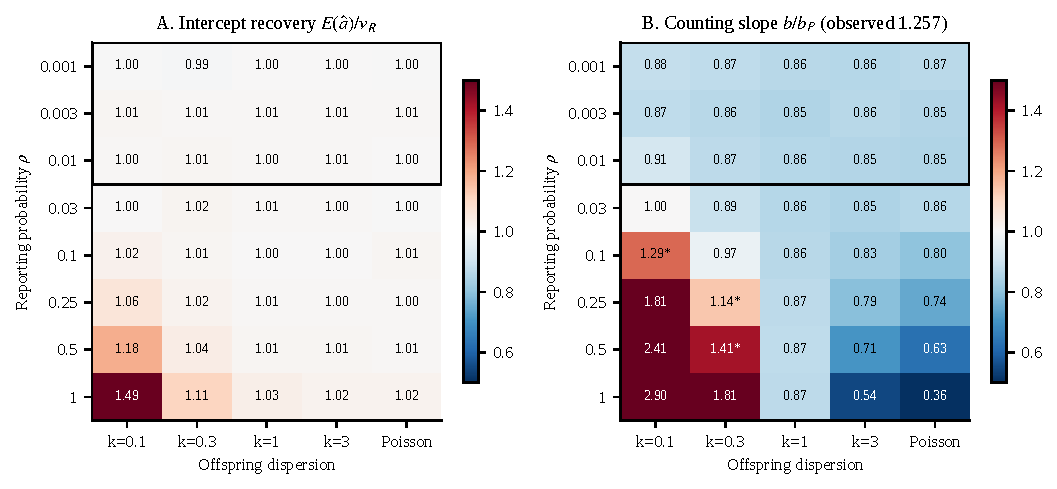
\includegraphics[width=0.98\linewidth]{figures/fig_07_rho_grid.pdf}
\caption{Reporting probability $\rho$ by offspring dispersion $k$, with independent transmission heterogeneity and 100 synthetic panels per cell on the real design. (A) Intercept recovery $\E(\hat a)/v_R$. (B) Mean counting slope relative to the independent-Poisson reference, $b/\bP$; asterisks mark cells whose Monte Carlo 2.5--97.5\% range contains the observed 1.257. The outlined rows mark the assumed range of $\rho$ for hospital admissions (0.001--0.01).}
\label{fig:rev-rho-grid}
\end{figure}

\subsection{Season intercepts}
\label{sec:res-season}

No difference between season intercepts was detected under the primary calibration (calendar-week permutation $p=0.102$; power 0.47 at the observed pattern). The Wald statistic was $W_{\mathrm{CGM}}=17.8$ on 3 degrees of freedom, and its calendar-week permutation $p$ was 0.102 (Monte Carlo standard error 0.003) (Table~\ref{tab:rev_season_calibration}; Fig.~\ref{fig:rev-season}B). Season statements below are therefore exploratory. The other calibrations disagree with one another. The asymptotic $\chi^2_3$ reference gave $p=0.0005$, the week-cluster wild bootstrap 0.011, the state-cluster wild bootstrap 0.013, the within-state permutation 0.045, generator-based references 0.005--0.055, the bootstrap-covariance statistic 0.138 and circular shifts of the season sequence 0.405. The state-level calibrations treat states as independent clusters although the season label varies only between weeks, and the generator-based ones depend on the simulated mechanism. Under the primary calibration, excluding the 2025 data-channel interruption gave $p=0.261$, restricting to rows with at least 90\% reporting coverage gave 0.081, and the fixed calendar windows for three seasons gave 0.031.

The 2023--24 intercept was the lowest, 0.0071 (two-way sandwich on the log scale, 0.0050--0.0100), against 0.0154--0.0180 in the other seasons (Table~\ref{tab:rev_season_effects}; Fig.~\ref{fig:rev-season}A). The ratio of the highest to the lowest intercept was 2.54 (season-stratified block bootstrap 1.75--4.35), an estimate that is biased upward. A contrast of 2023--24 against the other seasons, chosen after the data had been seen, gave a ratio of 0.43 (two-way sandwich on the log scale, 0.29--0.65) and is not tested. Power at the observed pattern was 0.47 (Monte Carlo standard error 0.025), and 80\% power would need a highest-to-lowest ratio of about 4.5 (Fig.~\ref{fig:rev-season}C). With equal season intercepts the test rejected in 0.0625 of simulated panels (Monte Carlo standard error 0.012), about one standard error above the nominal 0.05. This power curve uses a loss-level statistic whose permutation critical value, 17.65, is lower than that of the primary test, so it is probably optimistic. The absence of a detected difference is therefore weak evidence that the season intercepts are equal. With four seasons the design can detect only large differences, and the between-season variance itself cannot be estimated precisely (Appendix~\ref{app:seasons}).

Any season difference would be a difference in the combined transmission and reporting variation that the intercept reflects. Mean hospital reporting coverage of the sample rows was 90.9--94.2\% in every season (Table~\ref{tab:rev_season_effects}), but coverage does not measure the reporting probability per infection, and scaling counts by participation changed $a$ by 2.0\% (Section~\ref{sec:res-reporting}). Reporting regimes did differ outside the analysis windows: median participation in summer 2024, when reporting was voluntary, was 45.6\% against 92.3--94.2\% in the other summers (Table~\ref{tab:summer}).

\begin{table}[!tbp]
\centering
\scriptsize
\setlength{\tabcolsep}{3pt}
\caption{Equal-season-intercept test ($W_{\mathrm{CGM}}$ = 17.80): primary calibration of the locked plan and every secondary calibration}
\label{tab:rev_season_calibration}
\begin{tabularx}{\linewidth}{@{}X c c@{}}
\toprule
Calibration & $p$ (MCSE) & Draws \\
\midrule
Calendar-week permutation (primary, locked plan) & 0.102 (0.003) & 9,999 \\
Asymptotic $\chi^2_3$, sandwich $W$ & 0.0005 & -- \\
Asymptotic $\chi^2_3$, bootstrap-covariance $W$ & 0.138 & -- \\
Week-cluster wild bootstrap (Webb, null imposed) & 0.011 (0.001) & 9,999 \\
Circular shifts of the season sequence (exact, 42) & 0.405 & 42 \\
State-cluster wild bootstrap & 0.013 (0.002) & 2,000 \\
Within-state permutation & 0.045 (0.005) & 2,000 \\
Generator S1 (fixed transmission field) & 0.013 (0.006) & 400 \\
Generator S6 (fixed transmission field) & 0.045 (0.010) & 400 \\
Generator S8 (fixed transmission field) & 0.028 (0.008) & 400 \\
Generator S9 (fixed transmission field; post hoc law) & 0.005 (0.004) & 400 \\
Generator FD-S1 (redrawn per replicate) & 0.055 (0.016) & 200 \\
Generator FD-S8 (redrawn per replicate) & 0.050 (0.015) & 200 \\
Generator FD-S9-25 (redrawn per replicate; post hoc law) & 0.035 (0.013) & 200 \\
Generator FD-S9-50 (redrawn per replicate; post hoc law) & 0.045 (0.015) & 200 \\
Generator FD-S9-75 (redrawn per replicate; post hoc law) & 0.035 (0.013) & 200 \\
\midrule
\multicolumn{3}{l}{\emph{Data sensitivities, primary calibration (calendar-week permutation, $B$=9,999)}} \\
S-a6 exclude pause: $W$=11.04, 3 df, 36 weeks & 0.261 (0.004) & 9,999 \\
S-a8 coverage $\ge$ 90\%: $W$=16.77, 3 df, 42 weeks & 0.081 (0.003) & 9,999 \\
S-a4 calendar windows: $W$=15.55, 2 df, 29 weeks & 0.031 (0.002) & 9,999 \\
\bottomrule
\end{tabularx}
\par\smallskip\parbox{\linewidth}{\scriptsize\linespread{1.15}\selectfont Decision rule (locked analysis plan): significant only if the primary $p<0.05$. Verdict: not significant: season statements are exploratory/descriptive. Holm-adjusted over the two claims: E1 $<10^{-4}$, season 0.102. Shipped generator calibrations hold the transmission field fixed; S9 and FD-S9 laws were specified after the data were seen.}
\end{table}

\begin{table}[!tbp]
\centering
\scriptsize
\setlength{\tabcolsep}{3pt}
\caption{Season intercepts (reflecting transmission and reporting variation) with sandwich and season-stratified block-bootstrap intervals, and design-based power}
\label{tab:rev_season_effects}
\begin{tabularx}{\linewidth}{@{}l*{7}{>{\centering\arraybackslash}X}@{}}
\toprule
Season & Weeks & Rows & $a_s$ & 95\% CI (sandwich) & 95\% CI (bootstrap) & $a_s/a$ (95\% CI) & Coverage (\%) \\
\midrule
2022-23 & 9 & 365 & 0.0159 & 0.0112--0.0224 & 0.0102--0.0221 & 1.06 (0.68--1.64) & 90.9 \\
2023-24 & 12 & 499 & 0.0071 & 0.0050--0.0100 & 0.0050--0.0111 & 0.47 (0.34--0.71) & 94.2 \\
2024-25 & 8 & 356 & 0.0154 & 0.0092--0.0257 & 0.0084--0.0242 & 1.03 (0.59--1.55) & 93.8 \\
2025-26 & 13 & 528 & 0.0180 & 0.0108--0.0299 & 0.0090--0.0252 & 1.20 (0.71--1.56) & 92.3 \\
\midrule
\multicolumn{8}{l}{Highest/lowest intercept ratio 2.54 (bootstrap 1.75--4.35; biased upward)} \\
\multicolumn{8}{l}{Post hoc: 2023-24 vs geometric mean of the other seasons, ratio 0.43 (sandwich 0.29--0.65; bootstrap 0.31--0.72); no test} \\
\multicolumn{8}{l}{Design-based power at the observed pattern 0.47; minimum detectable highest/lowest ratio at 80\% power 4.48} \\
\bottomrule
\end{tabularx}
\par\smallskip\parbox{\linewidth}{\scriptsize\linespread{1.15}\selectfont Coverage: mean hospital-reporting coverage of the sample rows. Voluntary reporting May--Oct 2024; CDC data-channel pause 3 October to 13 November 2025.}
\end{table}


\begin{figure}[!tbp]
\centering
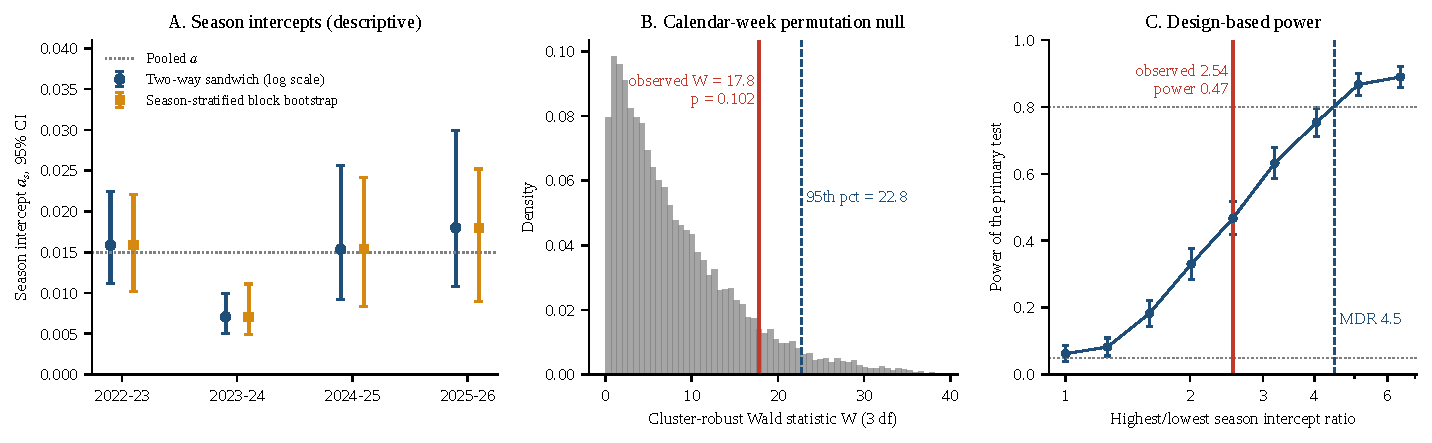
\includegraphics[width=0.98\linewidth]{figures/fig_08_season.pdf}
\caption{Season intercepts, exploratory. (A) Season intercepts $a_s$ in a model with a common slope. Intervals are two-way sandwich intervals on the log scale and season-stratified calendar-week block-bootstrap intervals, and the dotted line marks the pooled $a$. Panel (B) shows the calendar-week permutation distribution of the cluster-robust Wald statistic under equal season intercepts (9,999 permutations), with the observed statistic and the 95th percentile of the null distribution. Panel (C) shows the power of a permutation test at the 5\% level against the highest-to-lowest intercept ratio along the observed pattern. Error bars are binomial Monte Carlo errors, and MDR marks the minimum detectable ratio at 80\% power.}
\label{fig:rev-season}
\end{figure}

\subsection{Validity of the intervals}
\label{sec:res-validity}

Under generators that redraw the heterogeneity field in every replicate, the two-way interval covered the mean of $\hat a$ in 0.920--0.975 of panels, which meets SC4 (Table~\ref{tab:rev_generators}). Its mean standard error was 0.92--1.07 times the Monte Carlo standard deviation. Under mechanisms with reporting shocks the interval is centred on an estimator that falls short of the total (Section~\ref{sec:res-bias}), and it covered the true total in only 0.44--0.59 of panels, against 0.975 under independent heterogeneity. The observed standard error of $a$ was 1.53--2.08 times the Monte Carlo standard deviation under the fresh-draw laws of the plan and 1.39 under the national-share law with share 0.75, which was defined after the data had been seen. SC5 is therefore met only by a post hoc law. The two-way interval is wider than the Monte Carlo spread under every fresh-draw law, and the pigeonhole bootstrap standard deviation was 1.55--1.78 times it (Table~\ref{tab:r2-bootstrap-sd}), so the intervals reported here are conservative for the mean of $\hat a$ under these laws.

Generators built to reproduce the state structure of the panel did not close the gap between the variability of the data and of the simulated panels (Table~\ref{tab:r2-generator}). They combined a transmission field around a smoothed observed trend, with state-specific variance proportional to the population-dependent intercept or to state intercepts, clustered admissions and a reporting probability of 0.01 or 0.003. In five of the six cells the smoothed trend alone exceeded the transmission target, so the transmission standard deviation could not be calibrated. No cell reproduced all four tested features of the observed panel: the counting slope ratio fell inside the Monte Carlo range only without admission clustering, the 90th percentile of the count in five of six cells, the pooled-to-within-state slope ratio (T3) in none and the between-state spread of intercepts in all. Under these cells the two-way interval covered the mean of $\hat a$ in 0.96--1.00 of panels, the observed standard error was 1.63--2.31 times the Monte Carlo standard deviation, and the intercept captured 70--78\% of the simulated non-counting total, which the interval covered in only 0.015--0.16 of panels. Which features of the data inflate its variability relative to these mechanisms remains unexplained. Simulated null distributions for the season test, which drew on generators with a fixed heterogeneity field, gave $p$ values of 0.005--0.045; redrawing the field raised them to 0.035--0.055. These generator-based calibrations are not used as evidence for season differences.

\begin{table}[!tbp]
\centering
\scriptsize
\setlength{\tabcolsep}{3pt}
\caption{Fresh-draw generators (transmission field redrawn in every replicate, 200 panels each)}
\label{tab:rev_generators}
\begin{tabularx}{\linewidth}{@{}l*{9}{>{\centering\arraybackslash}X}@{}}
\toprule
Generator & MC SD of $\hat a$ & Observed SE / MC SD & Sandwich SE / MC SD & Coverage of $E(\hat a)$ & Coverage of true total & $E(\hat a)/v_R$ & $b/b_P$ & Week-centring reduction (\%) & Implied SD of $R$ (\%) \\
\midrule
FD-S1 & 0.00098 & 2.08 & 1.02 & 0.945 & 0.975 & 1.014 & 0.842 & 0.1 & 12.1 (9.8--14.7) \\
FD-S8 & 0.00127 & 1.60 & 0.92 & 0.920 & 0.440 & 1.749 & 1.281 & $-$0.8 & 9.2 (7.2--11.4) \\
FD-S9-25$^\dagger$ & 0.00130 & 1.56 & 0.94 & 0.925 & 0.520 & 1.754 & 1.298 & 8.3 & 9.2 (7.3--11.4) \\
FD-S9-50$^\dagger$ & 0.00132 & 1.53 & 1.03 & 0.940 & 0.570 & 1.753 & 1.297 & 18.4 & 9.2 (7.1--11.5) \\
FD-S9-75$^\dagger$ & 0.00147 & 1.39 & 1.07 & 0.975 & 0.590 & 1.731 & 1.310 & 26.9 & 9.3 (7.2--11.7) \\
\bottomrule
\end{tabularx}
\par\smallskip\parbox{\linewidth}{\scriptsize\linespread{1.15}\selectfont $^\dagger$ Post hoc law (national calendar-week share). SC5 (observed SE / MC SD in [0.67, 1.5] for some generator): met, only by a post hoc law; SC4 (coverage $\ge$ 0.90): met.}
\end{table}

